\documentclass[a4paper,onesided,12pt]{report}
\usepackage{styles/fbe_tez}
\usepackage[utf8x]{inputenc} % To use Unicode (e.g. Turkish) characters
\renewcommand{\labelenumi}{(\roman{enumi})}
\usepackage{amsmath, amsthm, amssymb}
 % Some extra symbols
\usepackage[bottom]{footmisc}
\usepackage{cite}
\usepackage{graphicx}
\usepackage{longtable}
\graphicspath{{figures/}} % Graphics will be here


% COVER PAGE
\title{THESIS TITLE}
\turkcebaslik{TEZ BAŞLIĞI}
\degree{B.S., Program Name, Boğaziçi University, 200000\\
	M.S., Program Name, Boğaziçi University, 2013}
\author{Name Surname}
\program{Your Program}
\subyear{2016}


\begin{document}

	\pagenumbering{roman}
	\makemstitle % M.S. thesis
	\tableofcontents
	%\listoffigures
	%\listoftables

  \clearpage

	\pagenumbering{arabic}
	\chapter{INTRODUCTION}
Evolution has been intensively studied since the publication of \emph{On the Origin of Species} in order to untie the mysteries behind fascinating machineries within living systems. In a broader sense, most of the studies on evolutionary biology have two main goals: (1) To document history of life through evolutionary point of view, and (2) to understand causal mechanisms responsible for the biological diversity that we have on Earth \cite{futuyma2001evolution, hird2017evolutionary}. In addition to these goals, the idea of using pre-existing living systems as cell factories for industrial purposes gained close attention in the last decades \cite{nielsen2016engineering}.

Evolutionary engineering, adaptive laboratory evolution in particular, refers to the experiments in which the environmental conditions are altered gradually to obtain adapted populations in the laboratories \cite{garland2009experimental}. Accumulation of mutations obtained due to environmental alterations through generations, where the favored individuals (mainly the ones with increased fitness) are selected to become parents of the next generation, result a population with advantageous traits compared to starting population. Challenges in the experimental design of evolutionary studies, such as maintenance of the organisms, controlling the environment, and feasibility to the omics analyses make the use of microorganisms more suited \cite{mcdonald2019microbial}.

% \section{Significance of Thesis}
The purpose of this thesis is to show metabolic changes in the adaptation of the yeast emph{Saccharomyces cerevisiae} using computational methods. Intracellular metabolic flux distributions obtained with the integration of transcriptomics data to the metabolic model of the yeast strains which evolved in various conditions such as high caffeine, high ethanol, high ions are going to be analyzed comparetively to the reference (unevolved) strains. This study will also contribute to the global understanding of metabolic regulations in the \emph{S. cerevisiae}, and will be further expandable into metabolic engineering studies of evolved strains.

\chapter{THEORETICAL BACKGROUND}

\section{Adaptive Laboratory Evolution}


\section{Systems Biology}
With the increasing availability of the computational tools and the development of high throughput techniques in the omics field, systems biology has shown a strong emergence in the last few years as a key multi-disciplinary field for integrating the multi-layer complexity of biological systems, particularly in the areas of transcriptomics, proteomics, metabolomics and fluxomics \cite{kitano2002systems}. This amount of available data allows researchers to investigate molecular cell processes in a large scales, applying theoretical, experimental and computational methods.

Biological systems based on complex interactions between various molecular components. The relations between these components are often obey nonlinear kinetics, for example, most of the reactions are regulated by one or more feedback or feed-forward loops with incomprehensible behaviours. When considered, cell structure and compartmentalization are also often introduce complexities to the unexpected behavior of the entire biological system \cite{bellouquid2006mathematical}. Mathematical modeling with these factors taken into consideration is used as a general approach to encompass existing knowledge in biological systems, and to gather information by analyzing these models to acquire a better understanding \cite{kremling2013systems}.

A mathematical model of a cell can be approached by two different approaches in either a bottom-up or top-down directionality (Figure \ref{fig:systemsbiology}) \cite{bruggeman2007nature, shahzad2012application}. Top-down approach is an experimental oriented approach, it starts from the whole picture and aims to characterize biological mechanisms closer to the smaller parts and their interactions in the network. In the bottom-up approach, collected data from biological knowledge is used as a starting point, a subsystem is generated to deduce the functional properties of smaller points in the network. Combination of the pathway level models (bottom-up) into a model for the entire system level (top-down) is the ultimate goal in the systems biology therefore these approaches are complementary.

\begin{figure}[ht]
\begin{center}
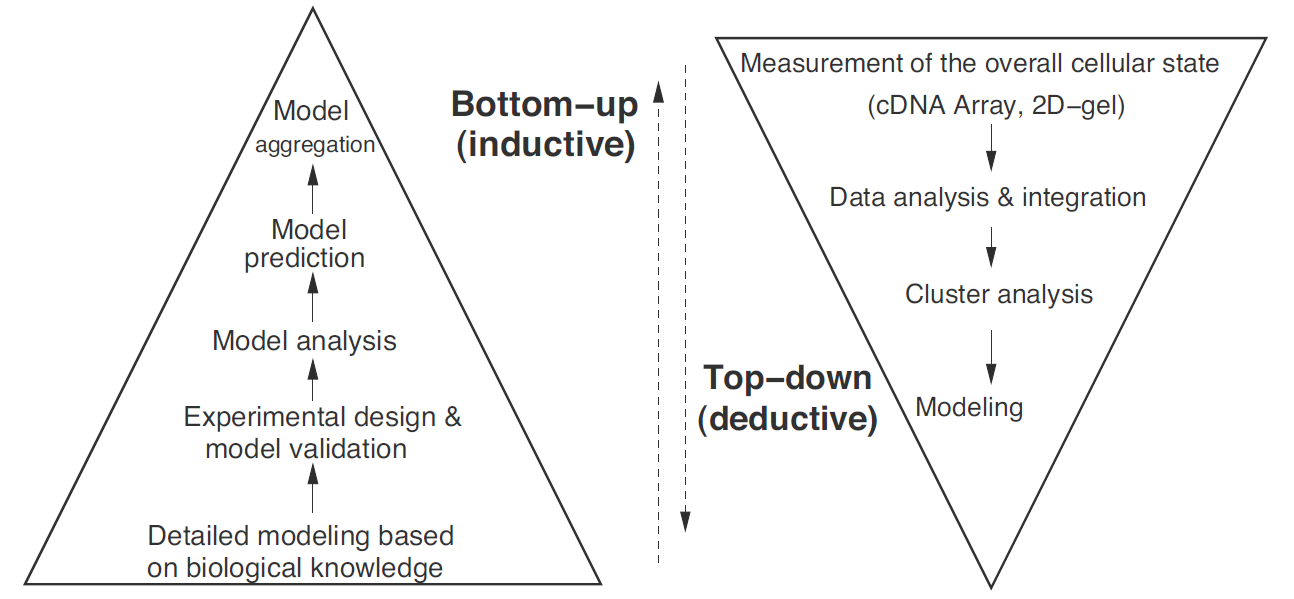
\includegraphics[width=0.8\columnwidth]{systemsbiology.png}
\end{center}
\caption[Systems biology approaches]{Systems biology approaches. Left: Bottom-up approach. Right: Top-down approach. Figure is taken from \cite{kremling2013systems}.}
\vskip\baselineskip % Leave a vertical skip below the figure
\label{fig:systemsbiology}
\end{figure}

\subsection{Metabolic Networks}
In the context of systems biology, metabolic network reconstructions have become a common interest for the researchers over the past 20 years \cite{thiele2010protocol}. Organism-specific metabolic network analyses allow scientists to design experiments and even obtain beforehand predictions. These networks are the main sources of the mathematical models which can simulate metabolic fluxes reflecting the experimantal reality \cite{orth2010flux}.

Before the improvement of genome sequencing or annotation technologies, initial core metabolic networks were based on the accessible information of biochemical pathways \cite{vallino1994carbon} \cite{varma1993biochemical}. In the last decade, larger genome-scale metabolic models (GSMMs) have been able to be developed rapidly with the help of databases for annotated genomes, providing information on substrates and products of each enzyme and each bioreaction \cite{feist2009reconstruction}. Growing biochemical databases provide automatization processes for the metabolic network reconstructions. As a result, genome-scale metabolic networks are available today for almost all organisms with an annotated genome available in the literature \cite{pitkanen2014comparative, kerkhoven2014applications}. From the first genome-scale metabolic model of \emph{Escherichia coli} to other organisms, the steps are required for GSMM development remained the same regardless of the biological diversity.

A generally applicable protocol is defined by the Palsson group \cite{thiele2010protocol, feist2009reconstruction} for the reconstruction of biochemical networks described in the Figure \ref{fig:modelreconstruction} \cite{chen2012metabolic}. Briefly, genomic data for the biochemical reactions of an organism are identified from the databases, such as NCBI, DDBJ and EMBL-EBI. Extraction and processing of the gene-protein-reaction relationship (GPR) of the genomic data results a draft reconstruction. GPR associations in the draft model should be reviewed by the researchers and manually curated if the identifying process is achieved with the help of automated computational algorithms \cite{pitkanen2014comparative}. Since the genomic data is the least representative of the biological phenotypes, available transcriptomic, proteomic, metabolomic and/or subcellular localization data are also used to further curate the model. Once the final metabolic network is reconstructed with bibliographic information, it is translated into a mathematical model.

\begin{figure}[ht]
\begin{center}
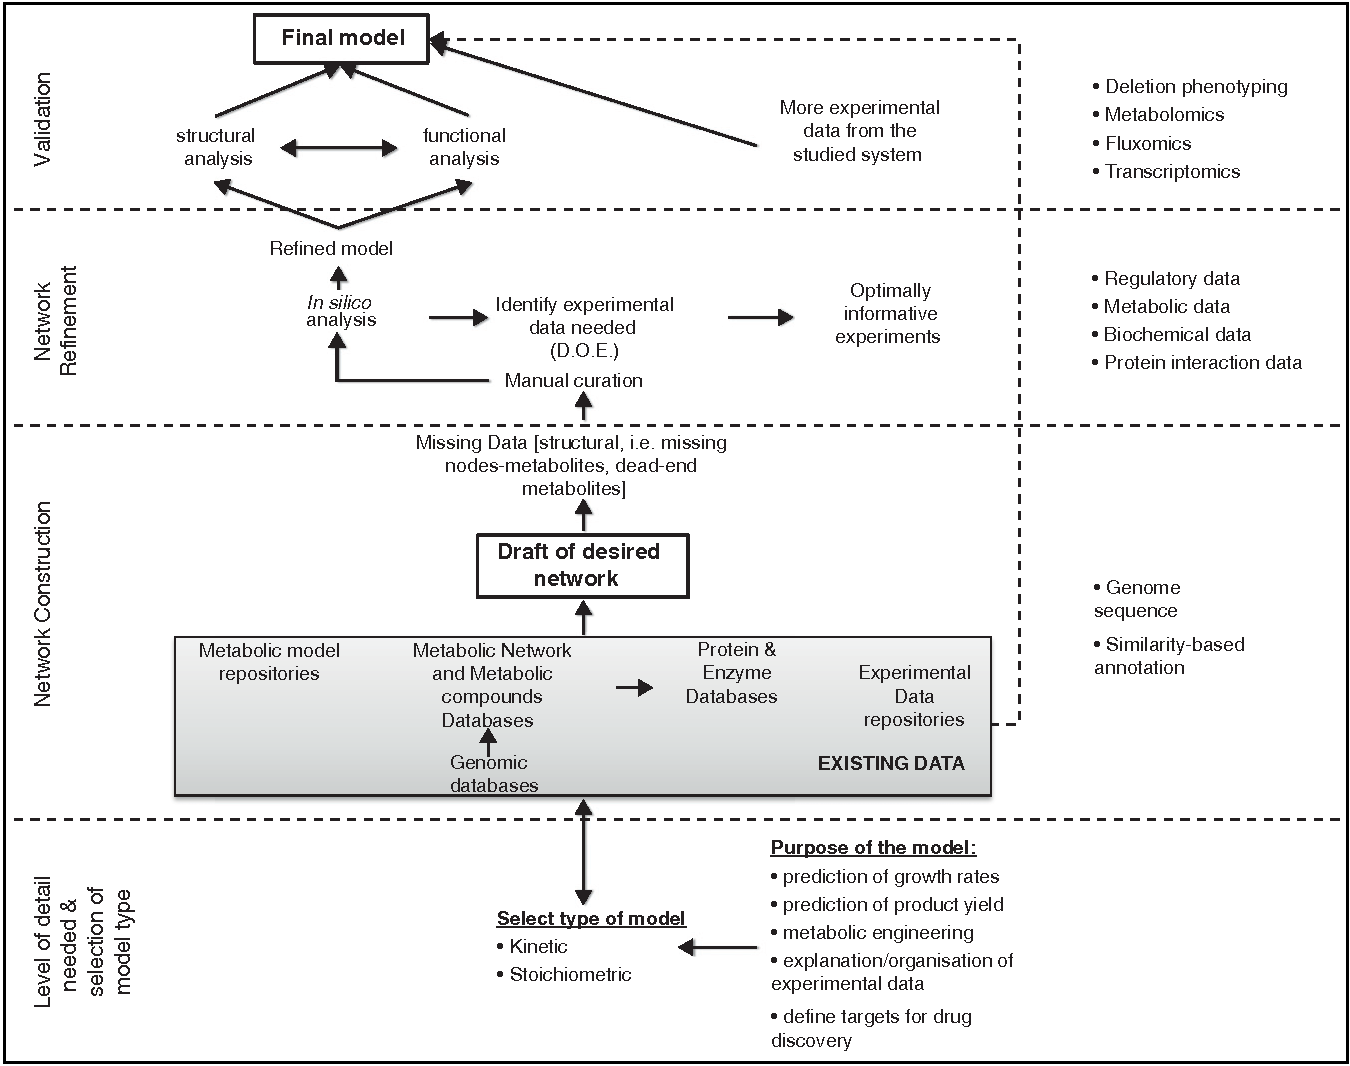
\includegraphics[width=1\columnwidth]{modelreconstruction.png}
\end{center}
\caption[Overview of metabolic network reconstruction protocol]{Overview of metabolic network reconstruction protocol. Figure is taken from \cite{chen2012metabolic}.}
\vskip\baselineskip % Leave a vertical skip below the figure
\label{fig:modelreconstruction}
\end{figure}

Once a metabolic network is reconstructed, a rational link between a genome sequence, the proteins encoded in the genome, and the reactions catalyzed by the proteins allowing to investigate the relationships between genotype and phenotype is achieved \cite{durot2008genome}. As the final step, GSMM needs to be validated by the new experimental data sets. GSMM validation process for various experimental conditions require detailed cultivation data from experiments. For example, information on the biomass composition of the specific organism leads more accurate biomass equation in the model, that is one of the key factors in the GSMM optimization and validation \cite{dikicioglu2015biomass}. Even tough multiple steps in the GSMM reconstruction can be achieved with the automated softwares available, it is usually necessary to curate the obtained model manually.

Approaches for analyzing metabolic networks are mainly categorized as dynamic or structural approaches. Even though the former is promising more realistic approach, its implementation in the literature is obstructed due to the unavailability of kinetic parameters for the majority of enzymes within a metabolic network \cite{machado2014systematic, ramkrishna2012dynamic} Because of the lack of kinetic parameters, structural metabolic modeling has been widely used for analyzing cellular metabolism at a steady-state assumption as a kind of snapshots taken at specific times.

GSMMs are one of the most useful tools in systems biology, especially in metabolic engineering studies \cite{kim2012recent}. In 1998, with the publication of \emph{Metabolic Engineering: Principles and Methodologies}, the term metabolic engineering is defined as the optimization of natural processes within cells to increase the production of certain substances \cite{stephanopoulos1999metabolic}. Hence, studies of metabolic engineering can be considered as genetic engineering in strain development. However, while metabolic engineering manipulates strains by altering flux distributions in the pathways; genetic engineering modificates specific genes, proteins and/or enzymes of interest \cite{stephanopoulos2012synthetic}. Although GSMMs are mainly used in metabolic engineering strategies, other applications both for descriptive and predictive purposes can be found in the literature \cite{osterlund2012fifteen}.

The ultimate goal of the GSMM reconstruction is to predict flux distribution profiles as close \emph{in silico} as they are \emph{in vivo}. Hence, GSMMs are in continuous research to improve predictability of organism-specific models.

\begin{figure}[ht]
\begin{center}
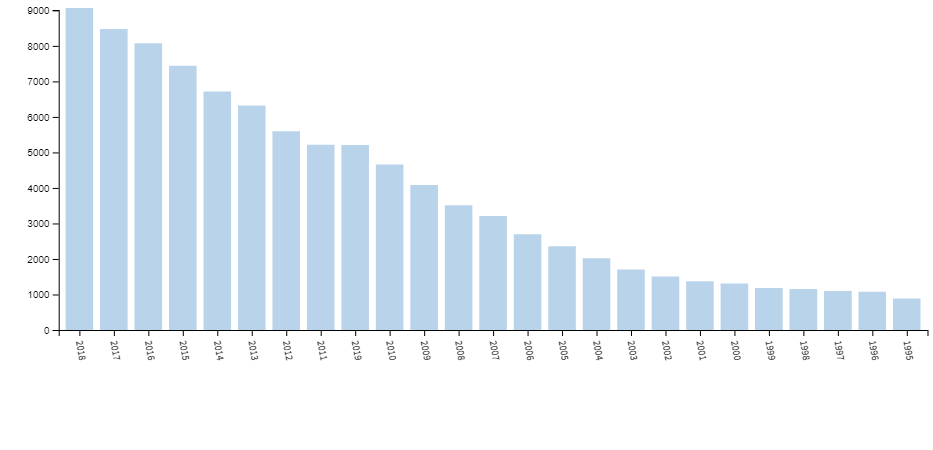
\includegraphics[width=1\columnwidth]{wos_metabolicmodel_search.jpg}
\end{center}
\caption[Web of Science artice counts on "metabolic model"]{Web of Science artice counts on "metabolic model"}
\label{fig:wos_metabolicmodel}
\end{figure}

\subsection{Mathematical Representation of Metabolic Networks}
\hl{In this section, there will be a review on} "Mathematical Framework Behind the Reconstruction and Analysis of Genome Scale Metabolic Models" \cite{pinzon2018mathematical}.

 This section will be detailed as much as possible since biology majors must understand the basics before reading the methods sections. How the biochemical equations are converted into differential equations? Steady state assumption, mass balances? Stoichiometric matrix formulation and its rank, linearly independent vectors, singular values? etc. Subjects will be similar to course ChE529.


\subsection{Constraint-Based Modeling}

\hl{In this section, there will be a review on} "Bringing genomes to life: the use of genome-scale in silico models" \cite{thiele2007bringing}.
Topics can be identification of constraints (physicochemical constraints, spatial constraints, environmental constraints, regulatory constraints), list of constraint-based modeling methods (optimal solutions, alternate optima, OptKnock, sampling as an unbiased modeling), linear programming, quadratic programming ...


\section{\emph{Saccharomyces cerevisiae}}

The species "yeast" includes a range of eukaryotic single-celled microorganisms, although it is commonly used to describe \emph{Saccharomyces cerevisiae}. Also known as the baker's yeast, \emph{S. cerevisiae} is one of the extensively used microorganisms for alcoholic fermentation of beverages, bio-ethanol production, and processing various foods since ancient times \cite{gelinas2009inventions}. It was the first eukaryotic organism whose genome was fully sequenced and annotated \cite{goffeau1997multidrug}, and besides its benefits in the industry, it is used as a model system for other eukaryotic cells including humans \cite{dujon1996yeast, botstein1997yeast}.

\subsection{Central Carbon Metabolism of \emph{S. cerevisiae}}
From the end of the eighteenth century, mainly after the fermentation is defined as "respiration without oxygen", the metabolism of \emph{S. cerevisiae} has been studied extensively \cite{barnett1998history, barnett2000history}. Its capability to produce ethanol is one of the most characterized microbial processes due to industrial utilization.

The set of anabolic and catabolic reactions in the cell are reffered as the metabolism. A shematic representation of the central carbon metabolism in \emph{S. cerevisiae} can be found in Figure \ref{fig:central_carbon_mech_of_s_cerevisiae_kegg}. Glycolysis, pentose-phosphate pathway (PPP), tricarboxylic acid cycle (TCA) or Krebs cycle, the glyoxylate cycle and the electron transport chain are the main pathways in central carbon metabolism.

 \begin{figure}[ht]
 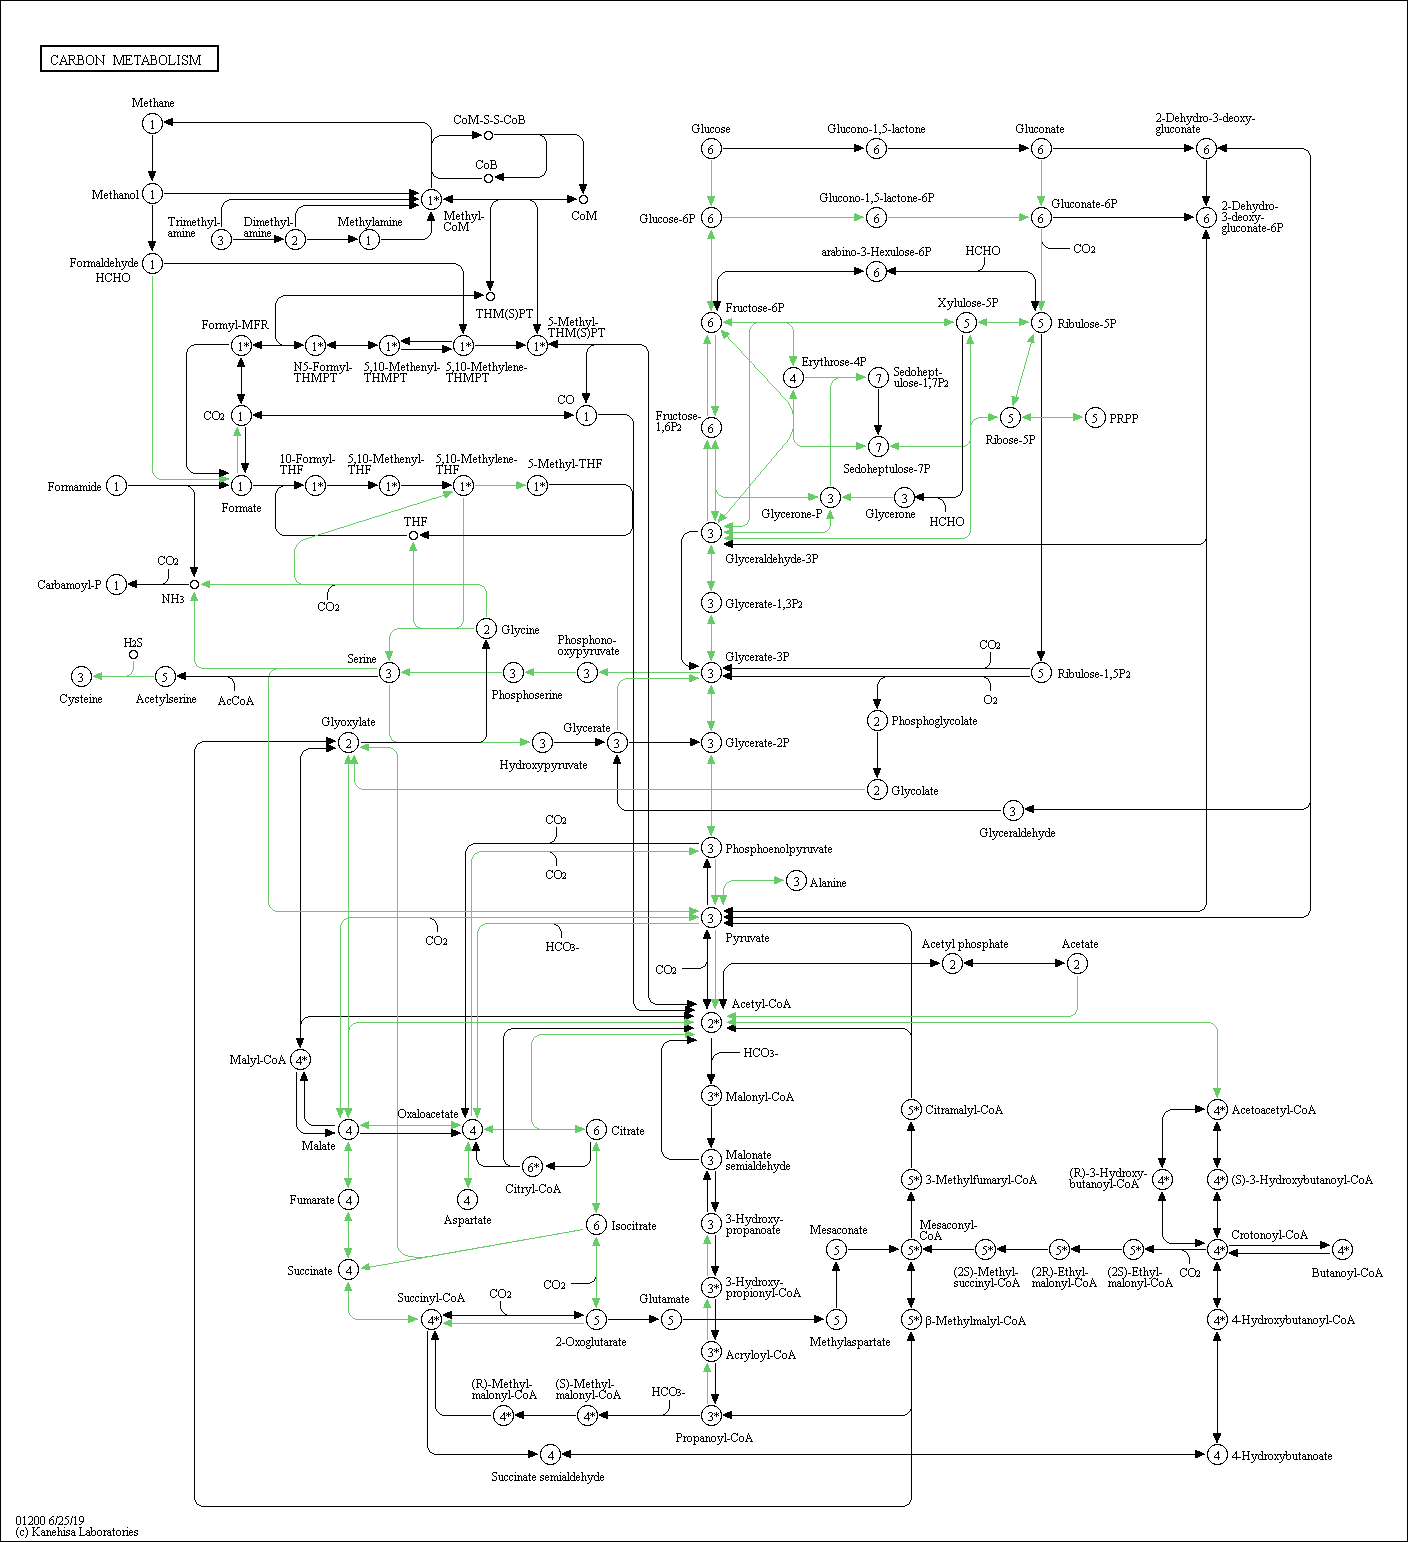
\includegraphics[width=1\columnwidth]{central_carbon_mech_of_s_cerevisiae_kegg.png}
 \caption[Central carbon mechanism of \emph{S. cerevisiae}]{Central carbon mechanism of \emph{S. cerevisiae} obtained from  KEGG \cite{kanehisa2000kegg}.}
 \vskip\baselineskip % Leave a vertical skip below the figure
 \label{fig:central_carbon_mech_of_s_cerevisiae_kegg}
 \end{figure}

\hl{In this section, there will be subsections on} all biological pathways individually (explaining each in detail -probably referencing Lehninger biochemistry-) especially NAD regulation, fermantation (crabtree effect, industrial applications, bio-ethanol production) etc... Maybe also regulation strategies in cells (feedback/feedforward loops with figures)

\subsection{Adaptive Evolution Studies on \emph{S. cerevisiae} (Palsson 2015)}

\subsection{Metabolic Models of \emph{S. cerevisiae}}
After the first \emph{S. cerevisiae} genome sequence is published, the first cDNA spotted microarray exploring metabolic gene regulation in 1997 \cite{derisi1997exploring}, and the first commercial platform for oligonucleotide microarray data (Affymetrix) to investigate cellular regulations were reported in 1998 \cite{cho1998parallel}. Existing genome data is integrated with the extensive annotation based on microarray data and biochemical knowledge from literature, leading of the publication of the first GSMM of \emph{S. cerevisiae} in 2013 \cite{forster2003genome}.   \hl{More in this section, there will be review on:} Genome-scale modeling of yeast: chronology, applications and critical perspectives \cite{lopes2017genome}

\subsection{Applications of \emph{S. cerevisiae} GSMMs}
 \hl{Literature review on the applications will be added.}

	\chapter{FLUX BALANCE ANALYSIS}

\section{Introduction}

\subsection{Understanding control in metabolic models}

Early enzymology assumed the existence of rate limiting steps in biological pathways. The intuition was that the overall rate of a pathway is constrained by the rate of the slowest step. As the slowest reaction rate increases the whole pathway rate increases in proportion until another step becomes limiting. Niederberger \emph{et. al} tested this assumption and found in contrast that individual up or down regulation of enzyme quantities at specific reaction steps had only marginal effect on overall tryptophan biosynthesis pathway in \emph{Saccharomyces cerevisiae}. The rate of the pathway was instead accelerated by increasing the quantity of five related enzymes in tandem. This research demonstrated control in a biological system is distributed over the system as a whole rather than concentrated at individual reactions.

The theory of metabolic control analysis (MCA)  states that there is no rate limiting step in a pathway, but instead each reaction shares a measure of overall control. The control the rate of reaction



	\bibliographystyle{styles/fbe_tez_v11}
	\bibliography{references}

\end{document}
